\documentclass[a4paper, 11pt]{article}
\usepackage[utf8]{inputenc}
\usepackage[T1]{fontenc}
\usepackage{amsmath, amsthm, amsfonts, amssymb, mathtools}
\usepackage{tikz}
\usetikzlibrary{arrows, positioning}
\title{perceptron}
\begin{document}
\maketitle
\section*{Introduction}
Perceptron is an elementary unit for neural networks.    
\begin{figure}
    % \caption{perceptron}
    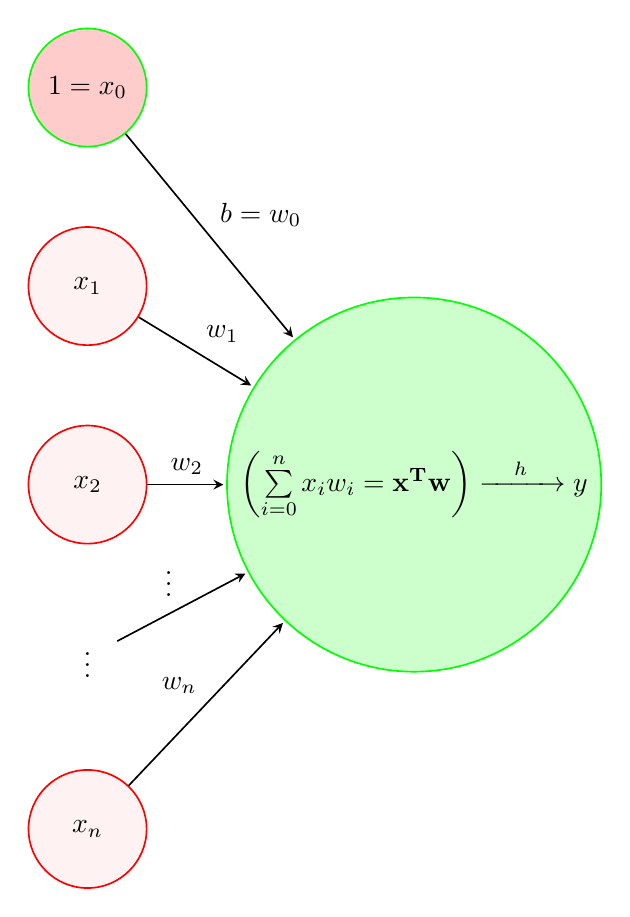
\begin{tikzpicture}[->,>=stealth, shorten >= 1pt, auto, node distance=1cm, semithick]
        \tikzstyle{input} = [circle, draw=red, fill=red!5, minimum size=15mm]
        \tikzstyle{ellipsis} = [circle]
        \tikzstyle{bias} = [circle, draw=green, fill=red!20, minimum size=15mm]
        \tikzstyle{output} = [circle, draw=green, fill=green!20]

        \node[bias](bias) {$1=x_0$};
        \node[input](input_1) [below=of bias] {$x_1$};
        \node[input](input_2) [below=of input_1]{$x_2$};
        \node[ellipsis](ellipsis) [below=of input_2]{$\vdots$};
        \node[input](input_n) [below=of ellipsis]{$x_n$};

        \node[output](wsum) [right=of input_2]{
            $\left(\sum\limits_{i=0}^{n} x_iw_i=\mathbf{x^T w}\right)\xrightarrow[ ]{\quad h \quad} y $};
        \path (bias) edge node {$b=w_0$} (wsum)
              (input_1) edge node {$w_1$} (wsum)       
              (input_2) edge node {$w_2$} (wsum)       
              (ellipsis) edge node {$\vdots$} (wsum)
              (input_n) edge node {$w_n$} (wsum);       
    \end{tikzpicture}
\end{figure}
\end{document}